\documentclass[a4paper,10pt]{article}
\usepackage[utf8]{inputenc}
\usepackage[final]{pdfpages}
\usepackage{caption}
\usepackage{fancyvrb}

\title{Math 660: Problem Set 6}
\author{Matthew Grasinger}

\begin{document}
  \maketitle

	\section{C1: Linear Iterative Methods} \label{sec:c1}
	
	\subsection{Source Code}
	
	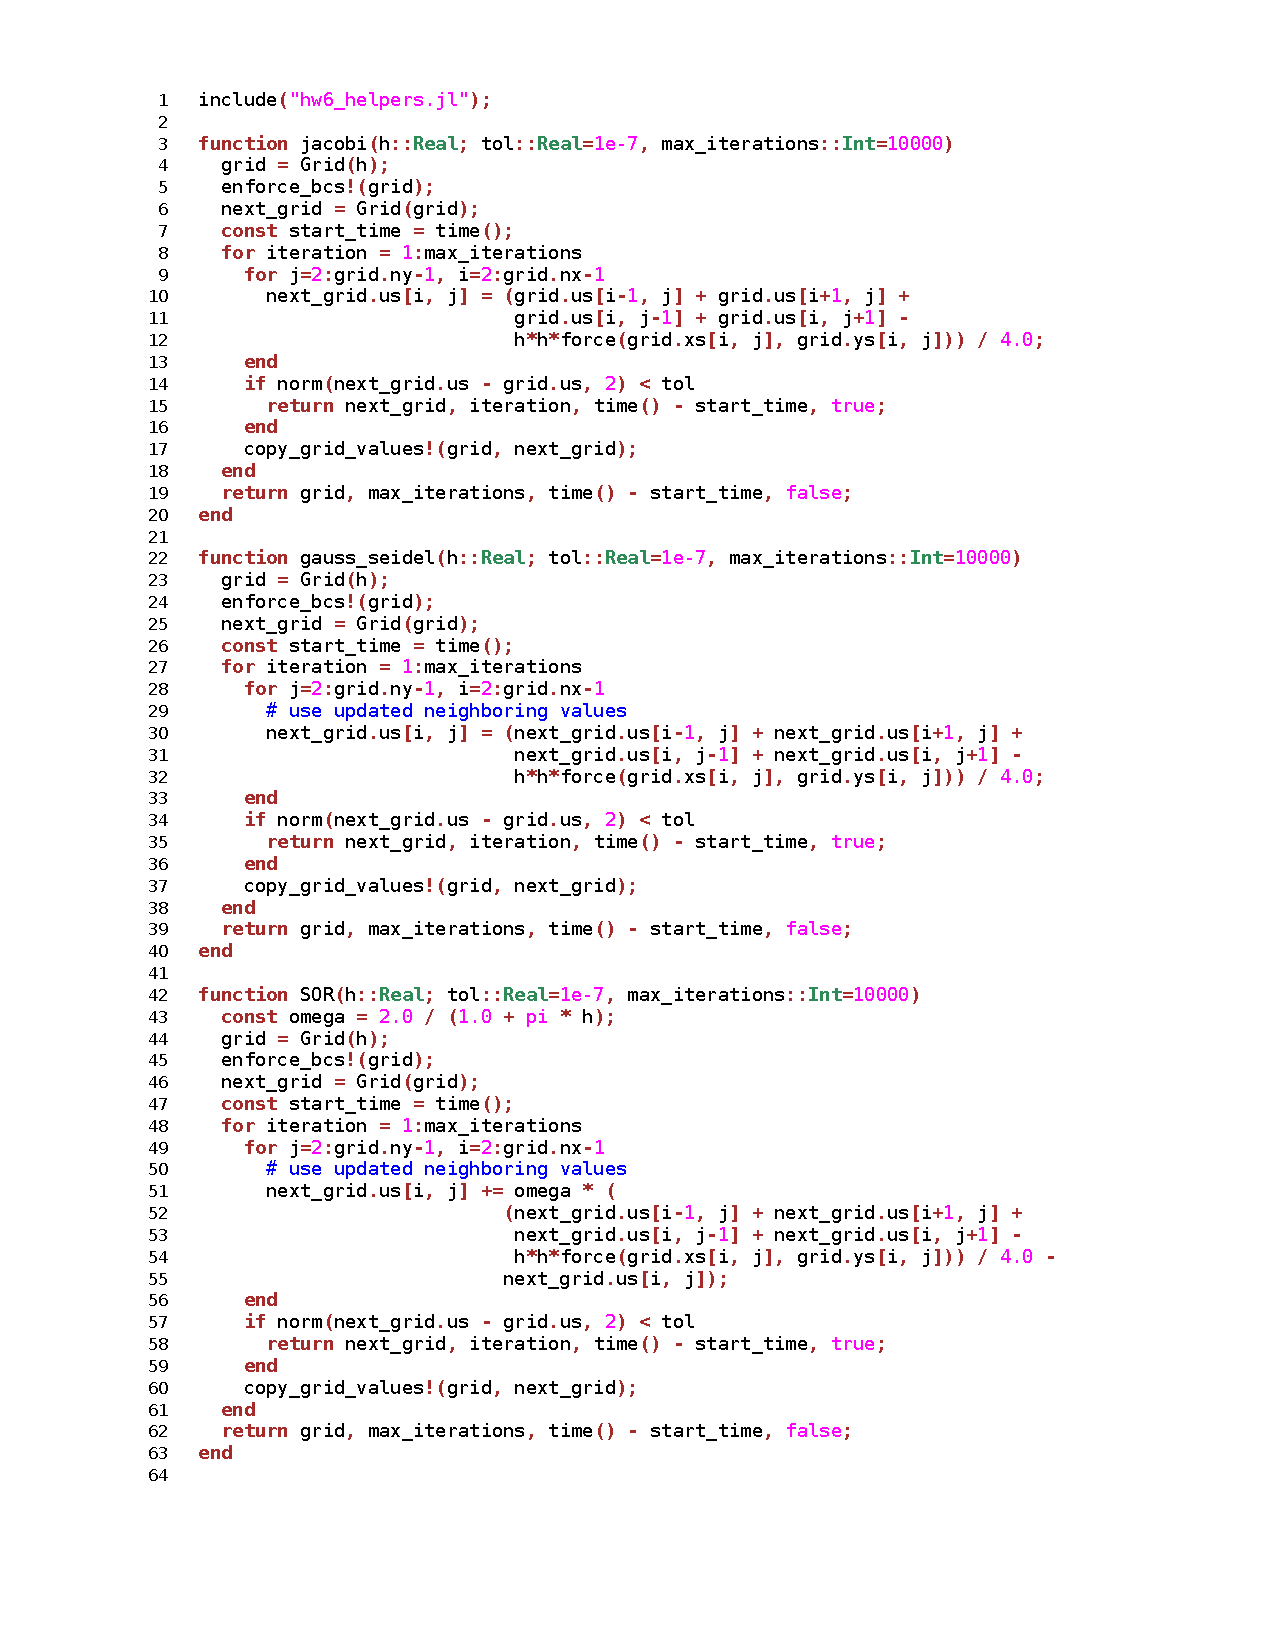
\includepdf[pages=-]{./c1.pdf}
	
	\subsection{Results}
	
	\VerbatimInput{c1.txt}
	
	\subsection{Discussion}
	
	The time per iteration was consistently on the order of $10^{-4}$--$10^{-5}$ seconds per iteration for each method, with longer times corresponding to finer grids.
	The fact that the time per iteration is consistent across methods agrees with theory.
	The accuracy, with respect to the analytical solution, is also consistent across methods and appears to depend primarily on the fineness of the grid.
	Therefore, the most apparent difference between methods is the number of iterations required to reach convergence.
	The Jacobi method required the largest number of iterations to converge.
	Gauss-Seidel converged in about half as many iterations on average.
	SOR converged consistently converged in the least number of steps, requiring an order of magnitude less steps than either the Jacobi or Gauss-Seidel methods.
	
	\section{C2: Conjugate Gradient}
	
	\subsection{Source Code}
	
	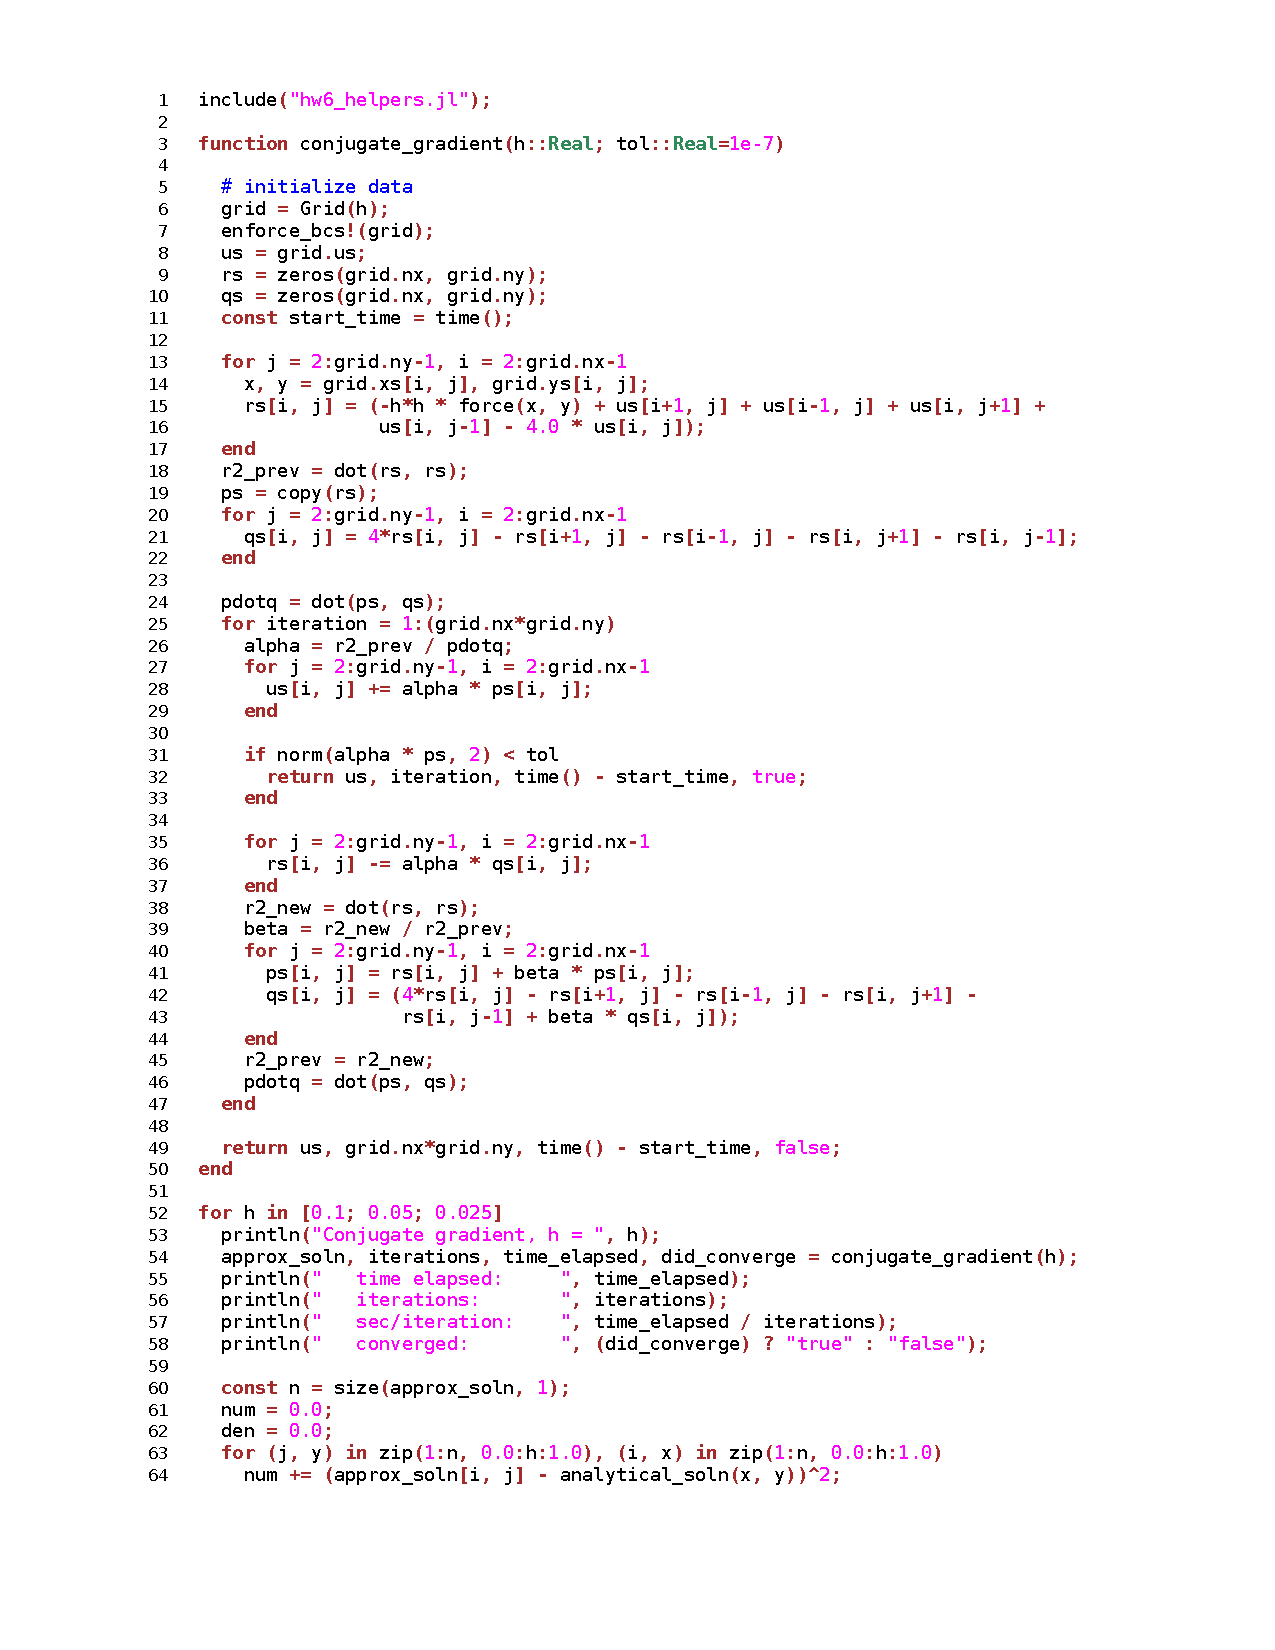
\includepdf[pages=-]{./c2.pdf}
	
	\subsection{Results}
	
	\VerbatimInput{c2.txt}
	
	\subsection{Discussion}
	
	The time per iteration was on the order of $10^{-4}$--$10^{-5}$ seconds per iteration for the conjugate gradient method, which is consistent with the methods used in Section \ref{sec:c1}.
	The accuracy, with respect to the analytical solution, was also consistent with the methods used in Section \ref{sec:c1}.
	However, the conjugate gradient required less iterations to converge for all cases.
	
\end{document}
